\documentclass[10pt,twocolumn]{article}

% ICML-style formatting (self-contained emulation, no external .sty)
\usepackage[letterpaper,margin=0.75in,columnsep=0.25in]{geometry}
\usepackage{times}
\usepackage{amsmath,amssymb}
\usepackage{booktabs}
\usepackage{graphicx}
\usepackage{caption}
\usepackage[hidelinks]{hyperref}
\usepackage{microtype}
\captionsetup{font=small,labelfont=bf}
\setlength{\abovecaptionskip}{4pt}

\title{\vspace{-4mm}\textbf{Volatility Risk Premia and High-Implied-Volatility Selection\\in CME G10 FX Options on Futures}}
\author{Nicholas Hong\\Nanyang Technological University\\\texttt{nhong001@e.ntu.edu.sg}}
\date{July 2026}

\begin{document}
\twocolumn[
\maketitle
\vspace{-8mm}
\begin{center}
\begin{minipage}{0.92\textwidth}
\small
\textbf{Abstract.}
We construct a research-grade panel of CME G10 FX options on futures from June 2010 to June 2026 and test whether option implied volatility systematically exceeds subsequent realized volatility. The dataset covers seven FX futures roots at 30, 60, and 90 day target tenors, built from Databento GLBX.MDP3 statistics and definition schemas. Two data contributions are documented: a correction for the 2017 CME FX options symbol migration, in which legacy American-style option families were replaced by European-style contracts under new symbols, and the removal of a structurally anomalous legacy NZD implied volatility regime that persists through 2013. Using Black-76 implied volatility and forward realized volatility computed from each option's own underlying futures contract, the final daily panel contains 70{,}714 root-tenor observations. A static short-volatility payoff proxy yields a mean implied-minus-realized spread of 0.28 volatility points (median 0.49, positive on 65.6\% of days) with a Newey-West 63-lag $t$-statistic of 1.79. Conditioning on high implied volatility through a leak-free cross-sectional selection rule nearly doubles the mean spread to 0.51 volatility points ($t_{\mathrm{NW63}}=2.41$, non-overlapping $t=2.71$), with monotone attenuation across selection ranks. Time-series threshold rules do not add value once look-ahead is removed from the conditioning signal. The payoff distribution is left-skewed in every variant and 2022 delivers losses across all seven currencies. All results are payoff proxies, not executable P\&L.
\end{minipage}
\end{center}
\vspace{4mm}
]

\section{Introduction}
Foreign exchange options embed expectations of future volatility, but they may also embed compensation for bearing volatility risk. If implied volatility (IV) is systematically higher than subsequently realized volatility (RV), option sellers earn a volatility risk premium (VRP) on average, in exchange for absorbing losses during volatility spikes. This paper asks three questions of CME G10 FX options on futures: (i)~does IV systematically exceed forward RV; (ii)~is the premium stronger when IV is high relative to its own history; (iii)~does a simple high-IV selection rule improve a short-volatility payoff proxy?

Our contribution is threefold. First, we build a cleaned, exchange-level CME FX options on futures dataset spanning 2010 to 2026, including a documented correction for the 2017 CME FX options symbol migration and the removal of an anomalous legacy NZD volatility regime; both corrections are necessary for any long-horizon study of these markets. Second, we compute Black-76 IV and forward RV from the specific underlying futures instrument referenced by each option, giving a contract-consistent VRP construction. Third, we test unconditional and conditional short-volatility payoff proxies with robust inference (Newey-West at multiple lags, non-overlapping sampling), a strictly leak-free conditioning signal, and full disclosure of all twelve strategy variants tested.

\section{Related Concepts}
The variance risk premium is defined as $\mathrm{VRP}_t = \mathrm{IV}_t^2 - \mathrm{RV}_{t,t+h}^2$; a positive value means a delta-hedged option seller collected more premium than the volatility paid out. Mechanisms that can sustain the premium include hedging demand from investors structurally long risk, crash-insurance demand, risk aversion to high-volatility states, limits to arbitrage and intermediary constraints, and compensation for the negatively skewed payoff of volatility selling. The FX setting is distinctive: there is no long-only anchor analogous to the equity premium, volatility is tightly linked to macro uncertainty, and safe-haven currencies (JPY, CHF) may carry structural volatility demand as macro hedges. Our finding that JPY commands the largest median VRP is consistent with that channel. The strategies tested connect to the literatures on variance risk premia, volatility timing, carry-style premia, and stress-regime reversals.

\section{Data}
\subsection{Source and coverage}
Data are Databento GLBX.MDP3 (CME Globex) statistics and definition schemas for FX options on futures and their underlying futures: roots 6A (AUD), 6B (GBP), 6C (CAD), 6E (EUR), 6J (JPY), 6N (NZD), 6S (CHF), from 2010-06-04 to 2026-06-08 in the final daily panel. Settlements are stat\_type~3 and open interest stat\_type~9; definitions supply instrument identifiers, expirations, strikes, option type, and the option-to-future link via \texttt{underlying\_id}.

\subsection{The 2017 symbol migration}
CME sunset the legacy American-style FX options families in mid-2017 and replaced them with expiration-only European-style contracts under new symbols (ADU, GBU, CAU, EUU, JPU, CHU for 6A, 6B, 6C, 6E, 6J, 6S; 6N unchanged). A naive symbol-based query shows an apparent post-2017 discontinuity. We use legacy roots before 2017-07 and migrated symbols (mapped back to economic roots) thereafter, excluding legacy non-6N symbols post-migration to avoid double counting.

\subsection{Cleaning and ATM selection}
Definitions are deduplicated per instrument (keep last by event time); settlements are deduplicated by (date, instrument). Options join to their own underlying future through \texttt{underlying\_id}, with 0\% unmatched across all 494 role-months. The clean panel holds 32{,}525{,}006 option-day rows across 193 monthly files. The ATM export requires positive settlements and strikes, 10--130 days to expiry, absolute log-moneyness at most 0.10, nearest-tenor assignment with outer-boundary ties, and the top 3 contracts per (date, root, tenor, type) bucket; after a global month-boundary deduplication it contains 440{,}467 rows.

\subsection{The 6N anomaly}
\label{sec:6n}
Legacy 6N settlements in 2010--2013 repeatedly imply 30--40\% volatility against roughly 8\% realized, exclusively on zero-open-interest contracts. Of 103 daily cells sample-wide with IV above 20\% and zero open interest, 102 are 6N cells in 2013; high-IV days for all other roots coincide with genuine stress (2011 euro area crisis, Brexit, SNB de-peg, COVID). 6N therefore enters the sample on 2014-01-01. Even in its clean sample, roughly 78\% of 6N daily cells carry zero open interest, a caveat retained on all 6N results.

\section{Methodology}
\subsection{Black-76 implied volatility}
Options on futures are priced with Black-76; carry is embedded in the futures price, so no separate rate inputs are needed for the volatility content:
\begin{equation}
C = e^{-rT}\left[F N(d_1) - K N(d_2)\right],
\end{equation}
\begin{equation}
d_{1,2} = \frac{\ln(F/K) \pm \tfrac{1}{2}\sigma^2 T}{\sigma\sqrt{T}},
\qquad T = \mathrm{DTE}/365.25,
\end{equation}
with $r=0$ in this pass (affecting only the premium discount factor). Pre-2017 legacy contracts are American-style, so Black-76 slightly overstates their IV, if anything inflating measured pre-2017 VRP. The solver inverts 440{,}462 of 440{,}467 ATM rows (99.999\%); 5 rows are below intrinsic value.

\subsection{Forward realized volatility}
For each option observation at date $t$ with target tenor $H \in \{30,60,90\}$ calendar days, RV is computed over $(t, t+H]$ from the settlement series of the option's \emph{own} futures contract, using log returns on consecutive settlements with a 14-calendar-day gap guard:
\begin{equation}
\mathrm{RV} = \sqrt{\frac{252}{n}\sum_{s \in (t,t+H]} r_s^2},
\end{equation}
where $n$ is the number of return observations. Each row carries a status flag; rows with insufficient span or observations (2{,}856 of 430{,}630, concentrated at the sample end) are excluded, leaving 427{,}774 valid option-level VRP observations (424{,}248 after the 6N exclusion). The volatility spread $\mathrm{IV}-\mathrm{RV}$ in annualized volatility points is the headline unit; option-level rows are aggregated equal-weight into a daily (date, root, tenor) panel of 70{,}714 rows.

\subsection{Strategy payoff proxies}
\label{sec:strat}
Twelve variants in three families are defined on the daily panel; the daily payoff proxy is the equal-weight mean $\mathrm{IV}-\mathrm{RV}$ spread of selected cells.
\textbf{Static}: all roots and tenors; 30d, 60d, 90d only; ex-6N; majors only (6E, 6B, 6J, 6S).
\textbf{Time-series signal}: sell cells whose IV $z$-score exceeds 0, 0.5, or 1. The $z$-score is leak-free: per root-tenor, $(\mathrm{IV}_t - \mu_{t})/\sigma_{t}$ where $\mu_t,\sigma_t$ are the rolling mean and standard deviation of the trailing 252 observations ending at $t-1$ (series shifted one day), minimum 126 observations.
\textbf{Cross-sectional}: per date and tenor, rank roots by the same $z$-score and sell the top 1, 2, or 3.
These are payoff proxies, not executable P\&L: bid-ask spreads, delta-hedging slippage, margin, and mark-to-market paths are excluded.

\section{Results}
\subsection{The premium by root and tenor}
Table~\ref{tab:root} reports medians by root and Figure~\ref{fig:ivrv} the IV/RV comparison. Median IV exceeds median forward RV for six of seven roots; the gap is largest for JPY (0.87 vol points), consistent with structural demand for yen optionality as a risk-off hedge, while NZD is flat and CHF positive but below average. Across tenors the premium is slightly stronger at the short end (medians 0.57, 0.50, 0.49 vol points at 30, 60, 90 days; positive on about 62.5\% of cells at each tenor).

\begin{table}[t]
\centering\small
\caption{Median implied volatility, forward realized volatility, and VRP spread by root (annualized \%, vol points). 6N from 2014.}
\label{tab:root}
\begin{tabular}{lccc}
\toprule
Root & Median IV & Median RV & Median IV$-$RV \\
\midrule
6A (AUD) & 9.84 & 9.36 & 0.56 \\
6B (GBP) & 7.98 & 7.78 & 0.64 \\
6C (CAD) & 7.00 & 6.68 & 0.53 \\
6E (EUR) & 7.55 & 7.30 & 0.51 \\
6J (JPY) & 9.07 & 8.21 & \textbf{0.87} \\
6N (NZD) & 9.33 & 9.81 & $-$0.03 \\
6S (CHF) & 7.71 & 7.44 & 0.39 \\
\bottomrule
\end{tabular}
\end{table}

\begin{figure}[t]
\centering
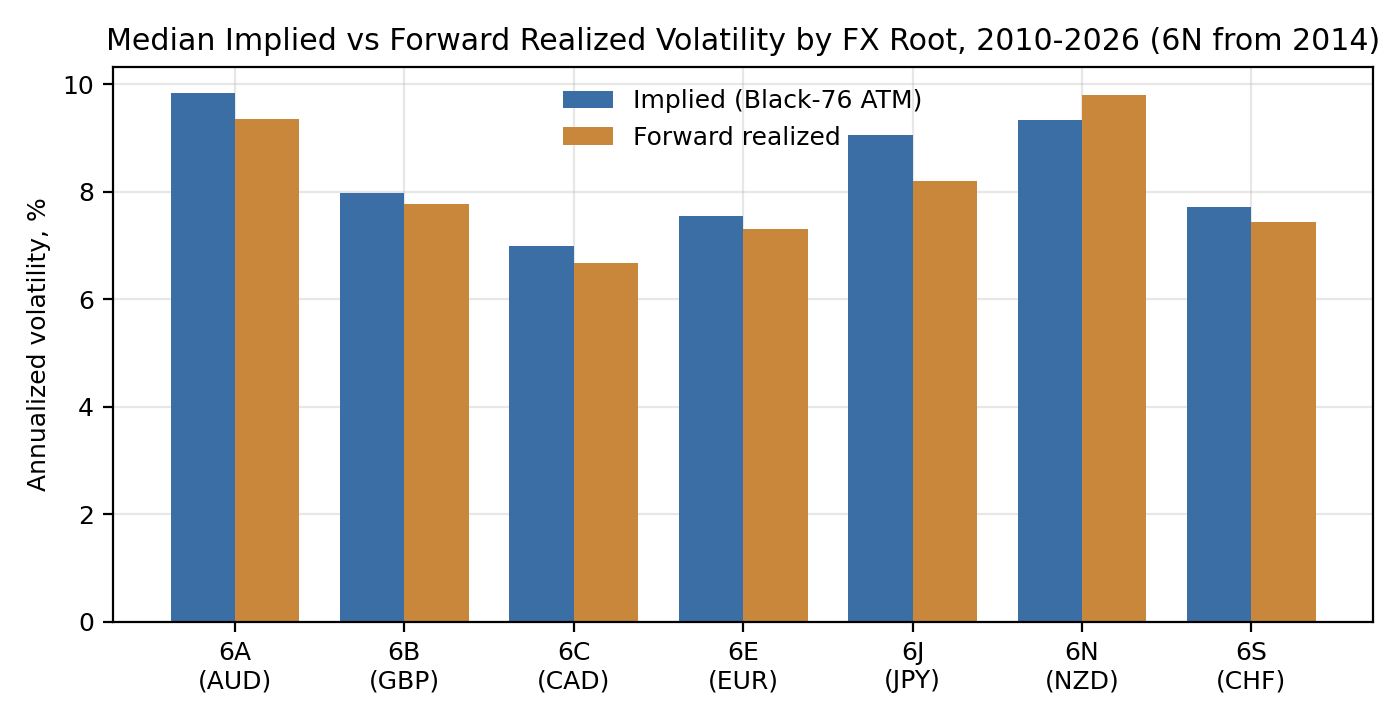
\includegraphics[width=\columnwidth]{figs/chart_1_iv_vs_rv_by_root.png}
\caption{Median implied vs forward realized volatility by FX root, 2010--2026 (6N from 2014).}
\label{fig:ivrv}
\end{figure}

\subsection{Yearly regimes}
Figure~\ref{fig:heat} shows yearly median VRP by root. The premium is strongly positive in 2010--2012, broadly negative across all seven roots in 2022 (from $-0.12$ for CAD to $-1.69$ for JPY), and recovers through 2023--2026. The 2022 reversal coincides with the fastest global hiking cycle in decades and large sustained currency trends. NZD shows sharply negative 2015--2016 (dairy collapse, RBNZ easing), subject to the thin-market caveat of Section~\ref{sec:6n}.

\begin{figure}[t]
\centering
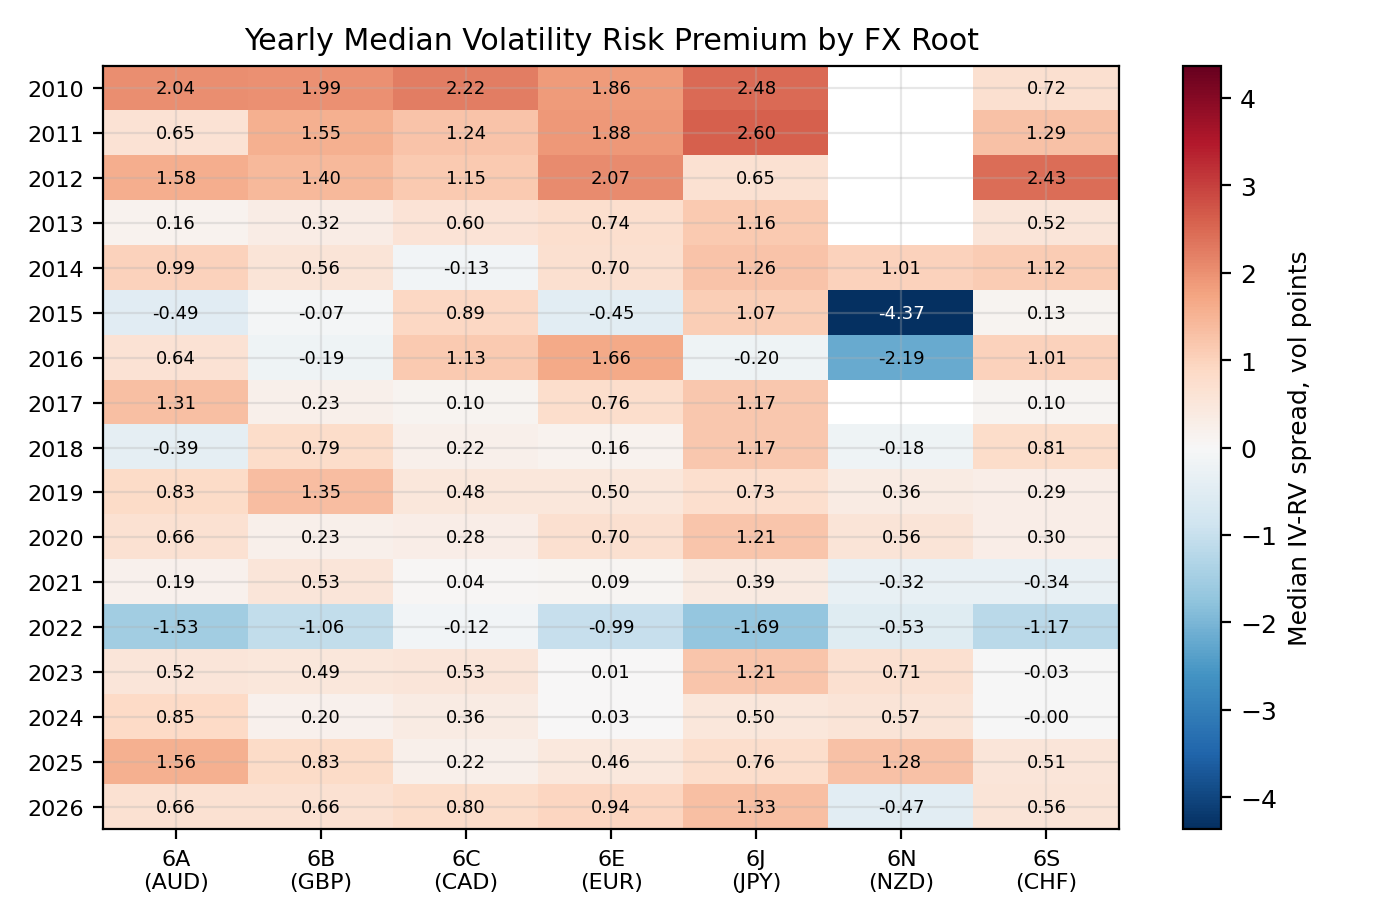
\includegraphics[width=\columnwidth]{figs/chart_4_yearly_vrp_heatmap.png}
\caption{Yearly median VRP spread by root (vol points).}
\label{fig:heat}
\end{figure}

\subsection{Strategy payoff proxies}
Table~\ref{tab:strat} reports all twelve variants. Four observations. First, the static premium is positive but marginal ($t_{\mathrm{NW63}}=1.79$; non-overlapping $t=2.27$); within the static family the 30-day tenor ($t=2.40$) and the ex-6N universe ($t=2.21$) are more robust. Second, cross-sectional high-IV selection nearly doubles the static mean (0.51 vs 0.28 vol points) with monotone attenuation through top-2 and top-3, the pattern expected if the effect is real rather than one lucky cell. Third, the time-series threshold family does not survive the leak-free $z$-score: means rise modestly but significance falls with the threshold. An earlier draft reported materially stronger conditional results; those were inflated by the 6N 2013 artifact of Section~\ref{sec:6n}, and their removal is a data correction, not a robustness choice. Fourth, skewness is negative in every variant (static: $-1.69$, excess kurtosis 7.0) and the mean sits well below the median throughout: frequent modest gains punctuated by large losses, with 2022 the clearest realization (Figure~\ref{fig:cum}).

Because the headline conditional rule is the best of twelve variants, its $t_{\mathrm{NW63}}=2.41$ overstates significance relative to a pre-registered test; we read it as suggestive evidence, supported by the monotone rank pattern, that cross-sectional high-IV conditioning helps.

\begin{table*}[t]
\centering\small
\caption{Strategy payoff proxies (vol points per day). NW63 is the Newey-West 63-lag $t$-statistic; NO21 is the mean simple $t$ over 21 non-overlapping subsamples. Payoff proxy: ex-post IV minus forward RV of selected positions; excludes transaction costs, hedging, and margin.}
\label{tab:strat}
\begin{tabular}{lrrrrrrrr}
\toprule
Strategy & N days & Mean & Median & Pos.\ \% & Skew & Ex.\ kurt & NW63 $t$ & NO21 $t$ \\
\midrule
static\_all\_roots\_all\_tenors & 3991 & 0.277 & 0.493 & 65.6 & $-1.69$ & 7.00 & 1.79 & 2.27 \\
static\_30d & 3808 & 0.306 & 0.530 & 65.9 & $-2.21$ & 11.44 & 2.40 & 2.32 \\
static\_60d & 3657 & 0.206 & 0.424 & 63.7 & $-1.75$ & 7.07 & 1.23 & 1.52 \\
static\_90d & 3191 & 0.162 & 0.391 & 61.0 & $-1.48$ & 5.03 & 0.82 & 1.09 \\
static\_ex\_6N & 3991 & 0.340 & 0.571 & 68.1 & $-1.81$ & 7.41 & 2.21 & 2.77 \\
static\_major\_roots\_only & 3991 & 0.319 & 0.618 & 67.2 & $-1.88$ & 7.48 & 1.93 & 2.38 \\
signal\_iv\_zscore\_ge\_0 & 2785 & 0.385 & 0.645 & 65.9 & $-1.84$ & 9.29 & 1.81 & 1.98 \\
signal\_iv\_zscore\_ge\_0p5 & 2215 & 0.378 & 0.647 & 64.6 & $-1.73$ & 8.55 & 1.50 & 1.53 \\
signal\_iv\_zscore\_ge\_1 & 1675 & 0.275 & 0.620 & 61.3 & $-1.61$ & 7.48 & 0.94 & 0.92 \\
xs\_top1\_iv\_z\_by\_date\_tenor & 3861 & \textbf{0.513} & \textbf{0.763} & 67.2 & $-2.33$ & 11.61 & \textbf{2.41} & \textbf{2.71} \\
xs\_top2\_iv\_z\_by\_date\_tenor & 3861 & 0.378 & 0.647 & 67.5 & $-2.97$ & 18.81 & 2.03 & 2.32 \\
xs\_top3\_iv\_z\_by\_date\_tenor & 3861 & 0.343 & 0.577 & 66.7 & $-2.30$ & 11.17 & 2.00 & 2.33 \\
\bottomrule
\end{tabular}
\end{table*}

\begin{figure}[t]
\centering
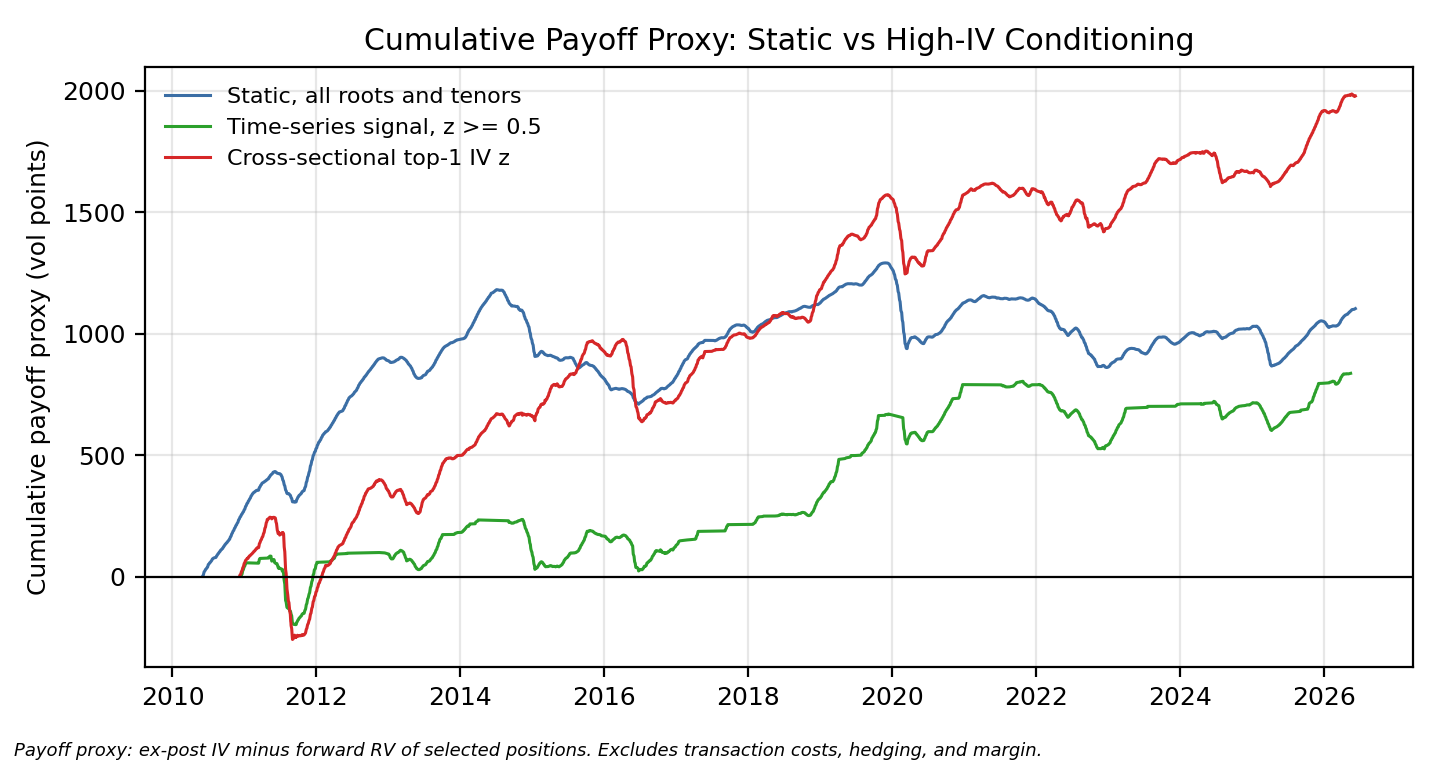
\includegraphics[width=\columnwidth]{figs/chart_6_cumulative_payoff.png}
\caption{Cumulative payoff proxy (vol points). Not an equity curve.}
\label{fig:cum}
\end{figure}

\section{Robustness}
\textbf{Newey-West.} Forward RV windows overlap across consecutive dates, so naive $t$-statistics are badly inflated: the best conditional strategy falls from a naive $t$ of 12.2 (NW5: 5.35) to $t_{\mathrm{NW63}}=2.41$; the static strategy from 10.4 to 1.79. We headline 63 lags (one quarter, matching the longest RV horizon).
\textbf{Non-overlapping sampling.} Sampling every 21st observation at all 21 offsets eliminates monthly-scale overlap by construction; the conditional strategy averages $t=2.71$ across offsets and the static strategy 2.27.
\textbf{6N exclusion.} 6N enters only from 2014 (Section~\ref{sec:6n}); the full-exclusion variant static\_ex\_6N is reported in Table~\ref{tab:strat} and is stronger than the all-roots static, as expected for a root with no measurable premium.
\textbf{Stress year.} 2022 is negative for all seven roots and should be read as an integral feature of the premium, not an anomaly.

\section{Limitations}
All results are payoff proxies, not executable P\&L. Transaction costs are excluded; measurement of resting-quote bid-ask spreads (stat\_types 7 and 8) is preliminary and pending, and plausible costs could consume much of the unconditional premium while leaving more headroom for the conditional spread. Delta-hedging slippage, margin, and capital are not modelled, so no Sharpe ratio is claimed. Pre-2017 legacy contracts are American-style approximated by Black-76. The rate is $r=0$. The panel is ATM-only (no smiles, risk reversals, or butterflies). The headline conditional rule is the best of twelve variants and its significance should be discounted for specification search. 6N carries a thin-market caveat throughout.

\section{Conclusion}
A cleaned 2010--2026 CME G10 FX options on futures dataset, corrected for the 2017 symbol migration and a legacy NZD data artifact, documents a persistent but time-varying volatility risk premium: strongest in JPY, absent in NZD, marginally significant unconditionally, and nearly doubled by a leak-free cross-sectional high-IV selection rule with monotone rank attenuation. The premium's left-skewed payoff and its broad 2022 reversal mark it as insurance compensation, collected steadily and repaid in concentrated stress regimes. Costs, hedging, and regime awareness are the natural next stage.

\vspace{2mm}
\noindent\textbf{Reproducibility.} Pipeline scripts (00--14), diagnostics, and a reproduction scorecard accompany this paper; all tables and figures regenerate from \texttt{vrp\_panel\_v3.parquet} via scripts 11--14.

\end{document}
